\documentclass[notes,slidesec,a4]{seminar}
\usepackage[spanish]{babel}
\usepackage[utf8]{inputenc}
\usepackage{fancybox}
\usepackage{graphics}
\usepackage{moreverb}
\usepackage{alltt}
\usepackage{html}
\usepackage{hthtml}
\usepackage{amsmath}
\usepackage[normalsize]{subfigure}
\usepackage{url}
\usepackage{listings}
\usepackage{eurosym}
\usepackage{t-gsyc-6}

%%--------------------------------------------------------------

\title{Seguimiento de rutas 3D por un drone con autolocalización
visual con balizas}
\author{Manuel Zafra Villar}

\cop{Manuel Zafra Villar}

\begin{document}
\maketitle


\begin{hslide}
\slsect{Contenidos}
\begin{itemize}
\item Introducción
\item Objetivos
\item Infraestructura
\item Componente de autolocalización
\item Componente de control de posición
\item Integración del sistema
\item Experimentos
\item Conclusiones
\end{itemize}
\end{hslide}



\begin{hslide}
\slsect{Introducción}
\end{hslide}



\begin{hslide}

\slsect{Objetivos}

Diseño de un sistema de navegación de para drones en espacios interiores mediante el seguimiento fino de una ruta en 3D. El drone debe conocer su posición en el entorno, para lo que se usará una técnica de visión artificial basada en marcadores.

\slsubsect{Subobjetivos}

\begin{itemize}
\item Refactorización e integración del componente \textit{Cam\_autoloc}
\item Desarrollo de un componente de control de posición
\item Validación experimental en entorno simulado
\end{itemize}

\end{hslide}



\begin{hslide}
\slsect{Infraestructura (I)}

\begin{itemize}
\item JdeRobot
	\begin{itemize}
	\item Pose3D
	\item Uav\_viewer
	\item Ardrone\_server
	\item CameraCalibrator
	\item Recorder/Replayer
	\end{itemize}
\item Gazebo
\item ICE
\item Parrot ArDrone2
\end{itemize}

\end{hslide}


\begin{hslide}
\slsect{Infraestructura (II)}

\begin{itemize}
\item AprilTags
\item Python
	\begin{itemize}
	\item NumPy
	\item PyQt
	\item PyOpenGL
	\item PyQtGraph
	\end{itemize}
\item OpenCV
\end{itemize}

\end{hslide}



\begin{hslide}
\slsect{Diseño global del sistema}

\begin{center}
	\begin{figure}
		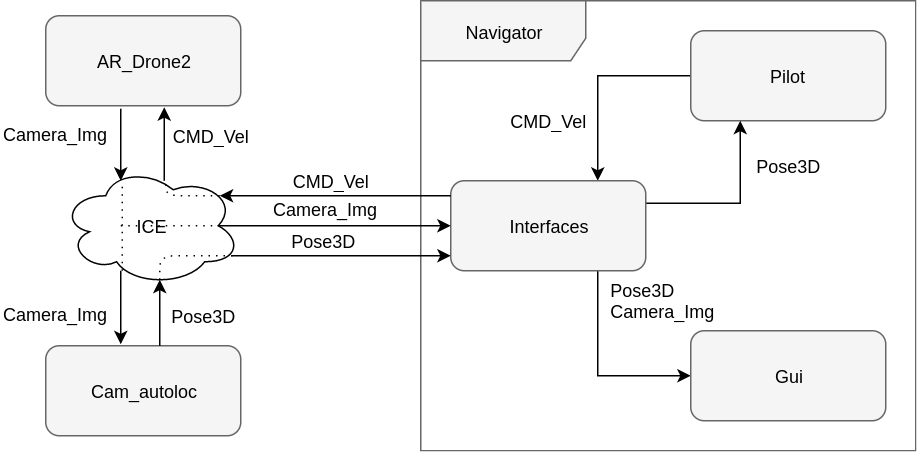
\includegraphics[width=11cm]{img/interactuacionproj2}
	\end{figure}
\end{center}

\end{hslide}



\begin{hslide}
\slsect{Componente de autolocalización}

\begin{center}
	\begin{figure}
		\centering
		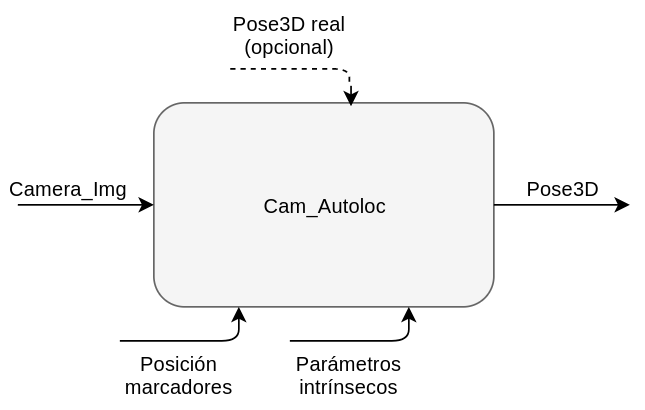
\includegraphics[width=8cm]{img/cam_autoloccaja}
	\end{figure}
\end{center}

\end{hslide}



\begin{hslide}
\slsect{Componente de control de posición}

\begin{center}
	\begin{figure}
		\centering
		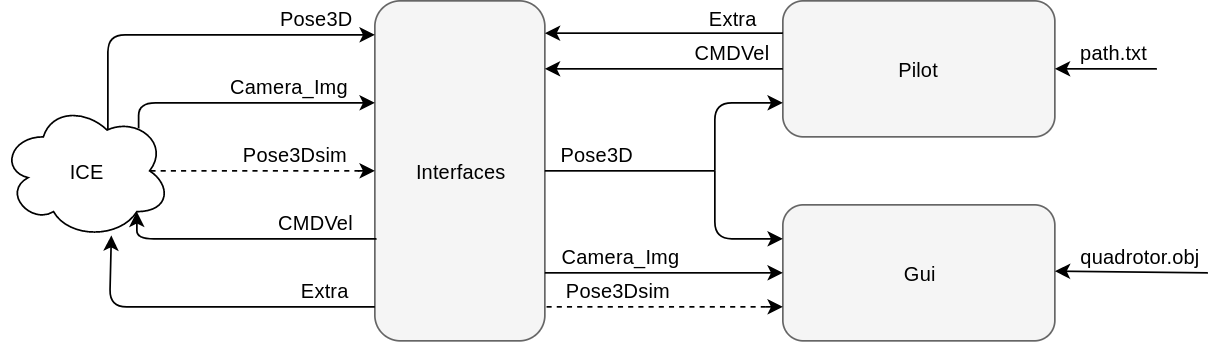
\includegraphics[width=12cm]{img/navigatorinter}
	\end{figure}
\end{center}

\end{hslide}


\begin{hslide}
\slsect{Integración del sistema}

\begin{center}
	\begin{figure}
		\centering
		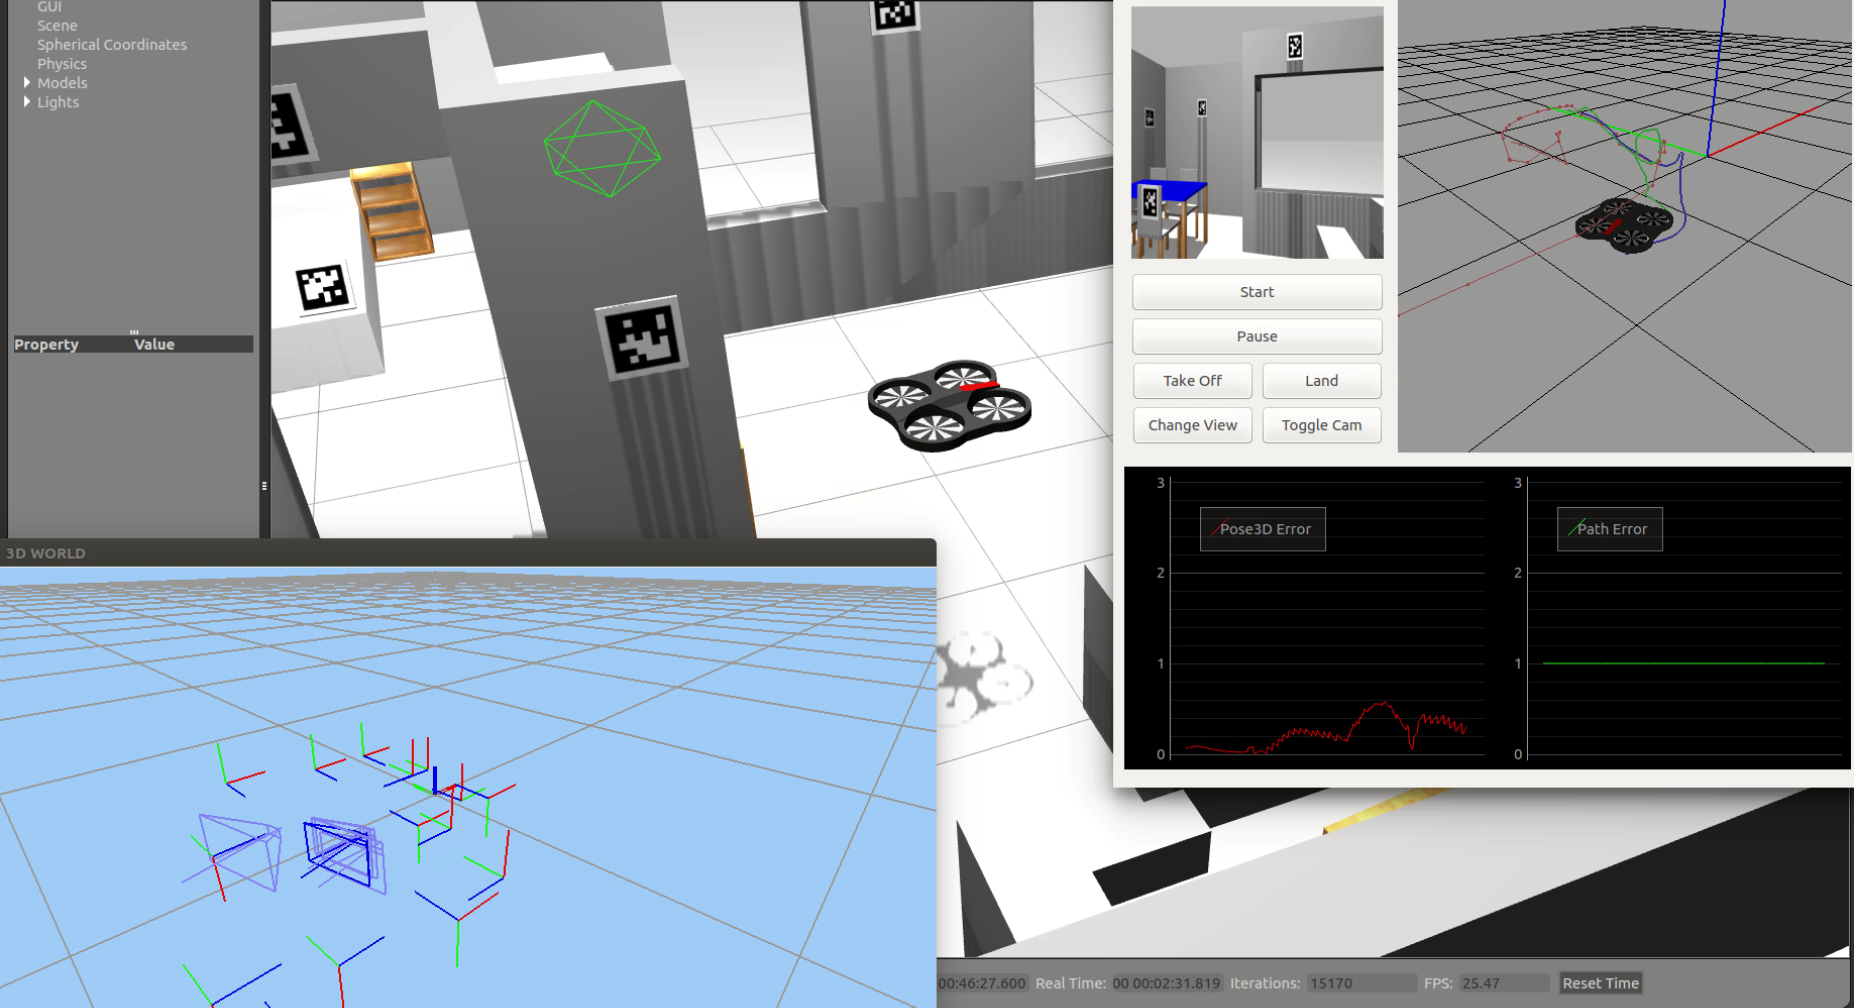
\includegraphics[width=10cm]{img/sistemacompleto}
	\end{figure}
\end{center}

\end{hslide}


\begin{hslide}
\slsect{Experimentos (I)}
\slsubsect{Entorno de simulación}

\begin{center}
	\begin{figure}
		\centering
		\begin{subfigure}
			\centering
			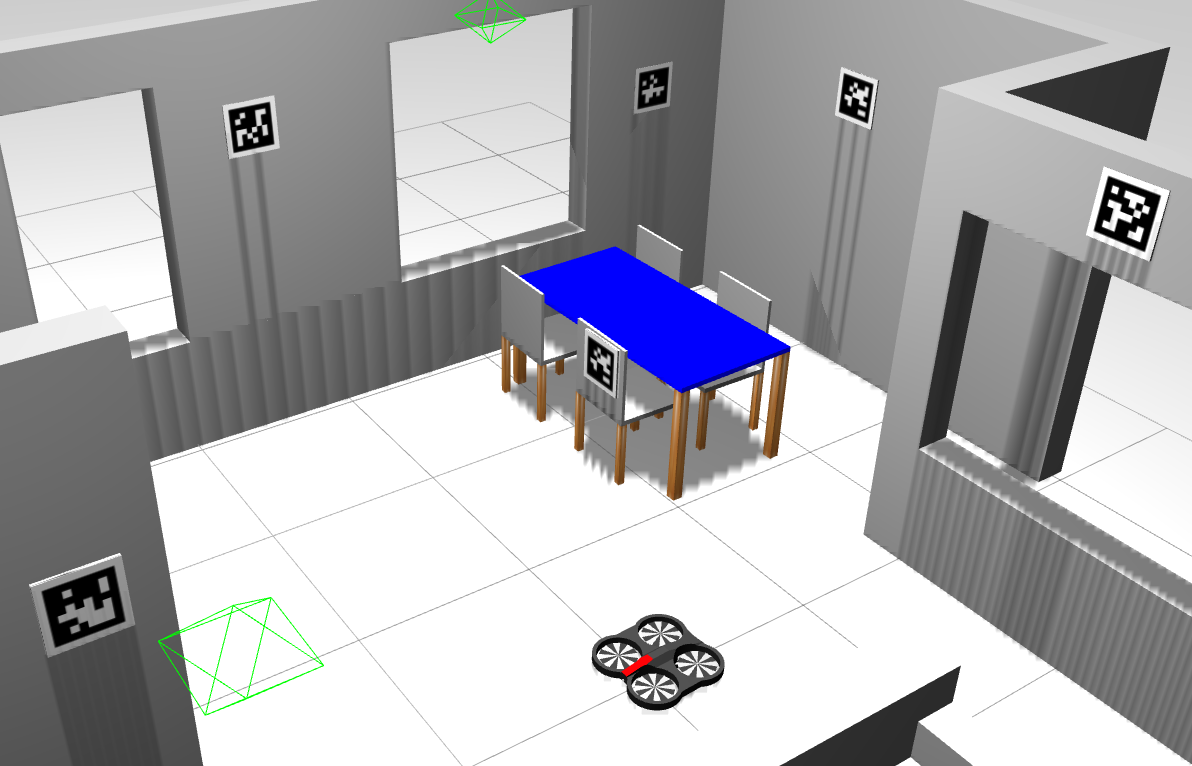
\includegraphics[width=5.45cm]{img/pisogazebo}
		\end{subfigure}%
		\begin{subfigure}
			\centering
			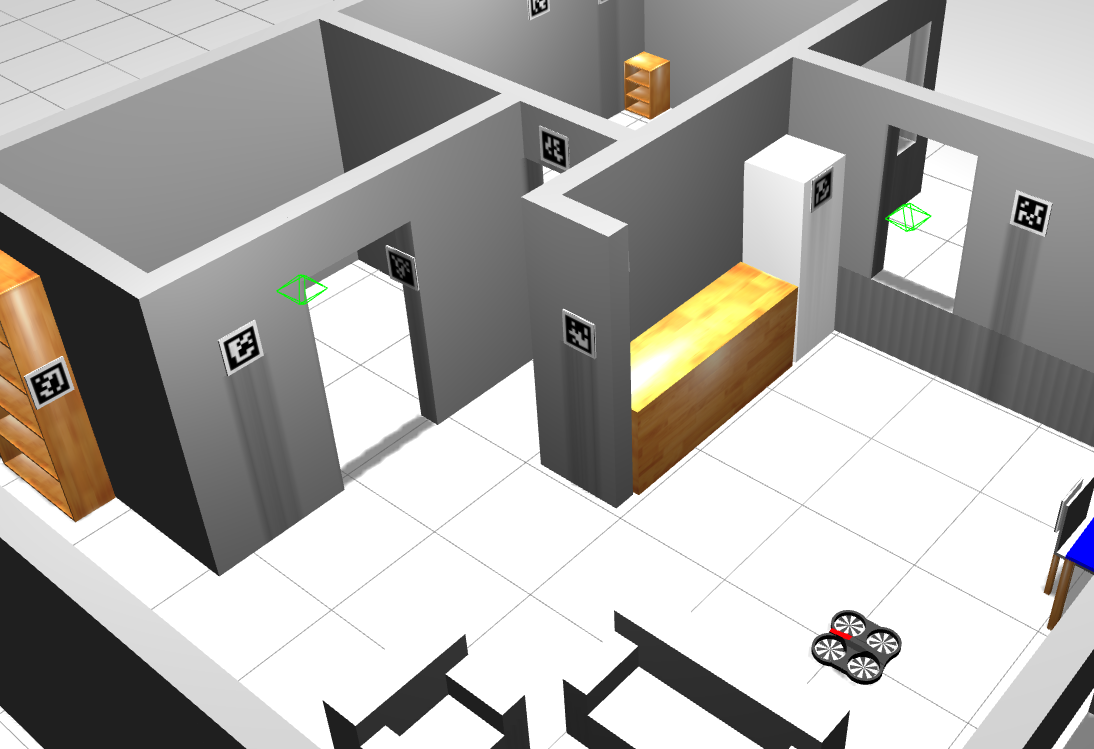
\includegraphics[width=5.12cm]{img/pisogazebo2}
		\end{subfigure}
	\end{figure}
\end{center}

\end{hslide}

\begin{hslide}
\slsect{Experimentos (I)}
\slsubsect{Control de posición con posición verdadera}

\begin{center}
	\begin{figure}
		\centering
		\begin{subfigure}
			\centering
			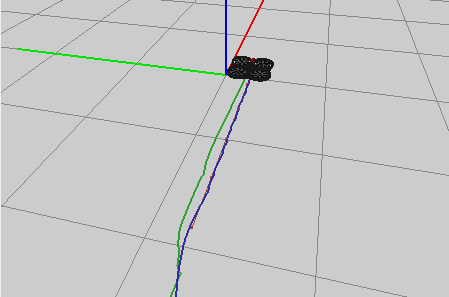
\includegraphics[width=5cm]{img/testlinearecta}
		\end{subfigure}%
		\begin{subfigure}
			\centering
			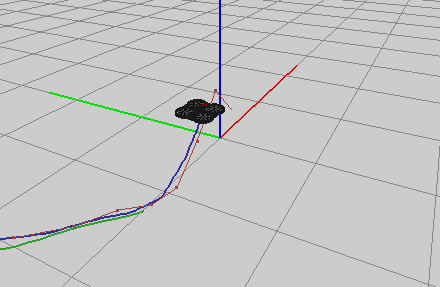
\includegraphics[width=5.1cm]{img/rutacambiosaltura}
		\end{subfigure}
	\end{figure}
\end{center}

\end{hslide}


\begin{hslide}
\slsect{Experimentos (I)}
\slsubsect{Control de posición con posición verdadera}

\begin{center}
	\begin{figure}
		\centering
		\begin{subfigure}
			\centering
			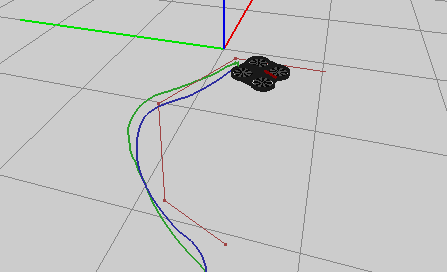
\includegraphics[width=5cm]{img/rutacurvas}
		\end{subfigure}%
		\begin{subfigure}
			\centering
			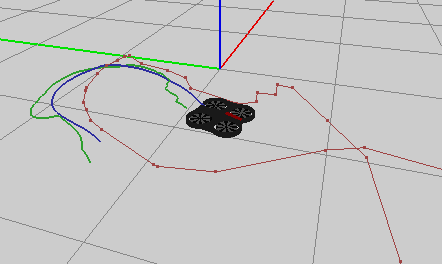
\includegraphics[width=5.13cm]{img/rutacompleja}
		\end{subfigure}
	\end{figure}
\end{center}

\end{hslide}


\begin{hslide}
\slsect{Experimentos (I)}
\slsubsect{Componente de autolocalización}

\begin{center}
	\begin{figure}
		\centering
		\begin{subfigure}
			\centering
			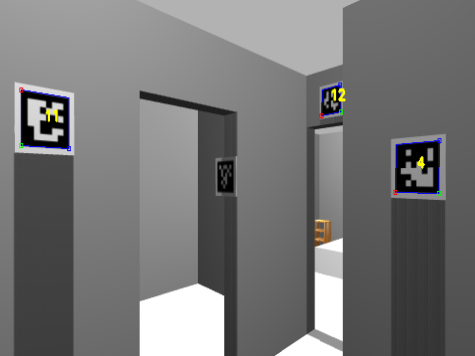
\includegraphics[width=3.5cm]{img/pisoloc2cam}
		\end{subfigure}%
		\begin{subfigure}
			\centering
			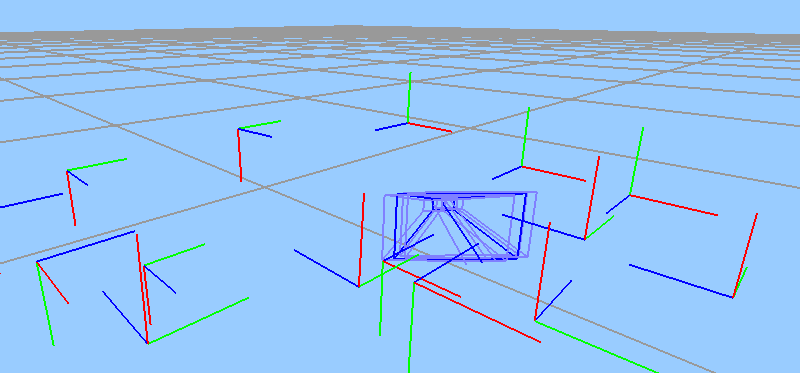
\includegraphics[width=7cm]{img/pisoloc2}
		\end{subfigure}
	\end{figure}
\end{center}	

\end{hslide}


\begin{hslide}
\slsect{Experimentos (I)}
\slsubsect{Componente de autolocalización}

\begin{center}
	\begin{figure}
		\centering
		\begin{subfigure}
			\centering
			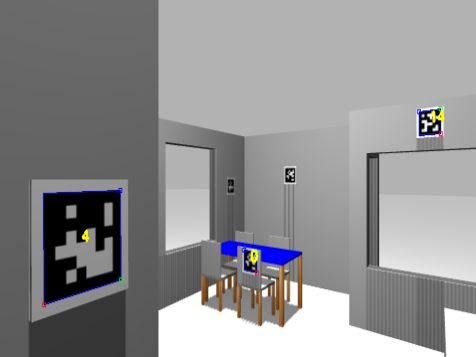
\includegraphics[width=3.5cm]{img/pisoloc3cam}
		\end{subfigure}%
		\begin{subfigure}
			\centering
			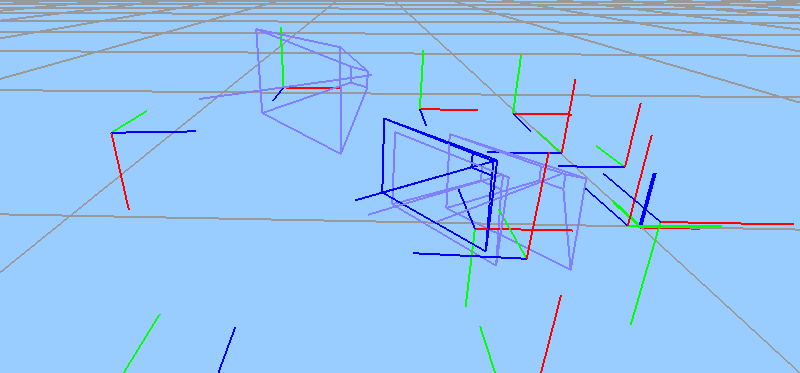
\includegraphics[width=7cm]{img/pisoloc3}
		\end{subfigure}
	\end{figure}
\end{center}

\end{hslide}


\begin{hslide}
\slsect{Experimentos (I)}
\slsubsect{Sistema completo}

\begin{center}
	\begin{figure}
		\centering
		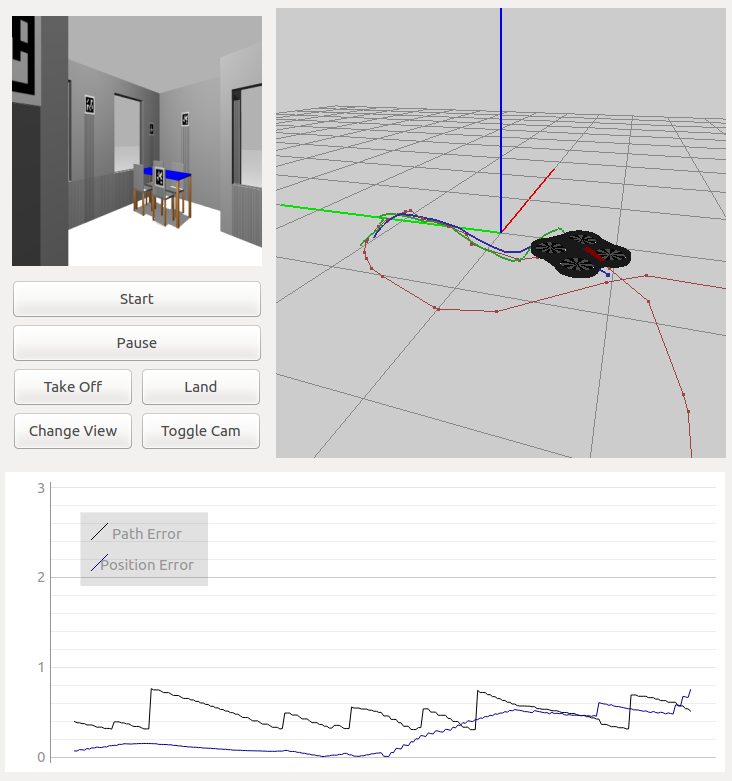
\includegraphics[width=5.1cm]{img/fulltest2}
	\end{figure}
\end{center}

\end{hslide}


\begin{hslide}
\slsect{Experimentos (I)}
\slsubsect{Sistema completo}

\begin{center}
	\begin{figure}
		\centering
		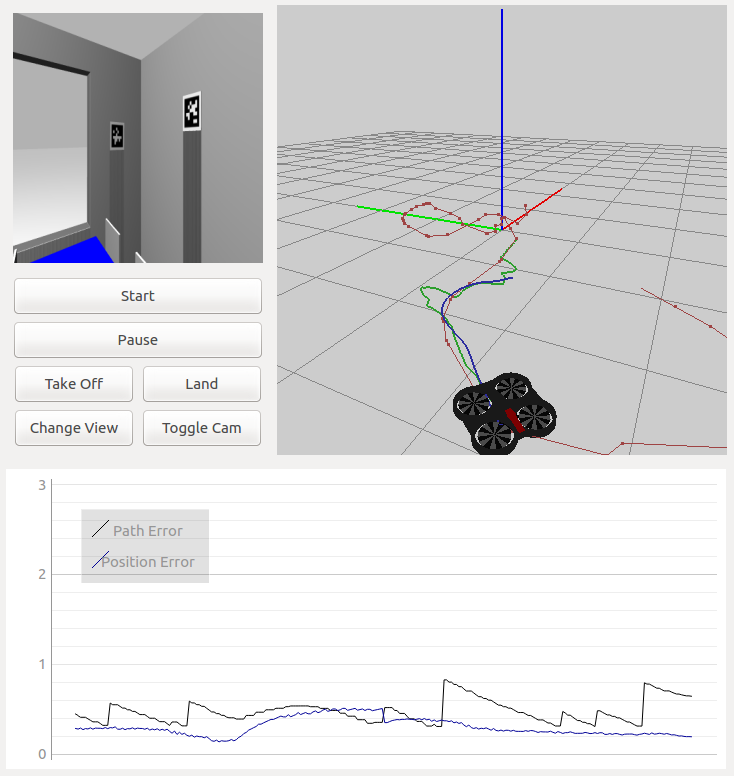
\includegraphics[width=5.1cm]{img/fulltest3}
	\end{figure}
\end{center}

\end{hslide}


\begin{hslide}
\slsect{Experimentos (II)}
\slsubsect{Componente autolocalización en entorno real}

\begin{center}
	\begin{figure}
		\centering
		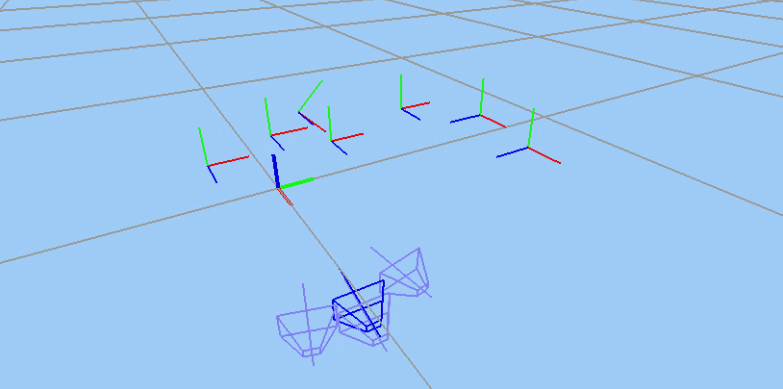
\includegraphics[width=9cm]{img/loc4m}
	\end{figure}
\end{center}

\end{hslide}


\begin{hslide}
\slsect{Experimentos (II)}
\slsubsect{Sistema completo en entorno real}

\begin{center}
	\begin{figure}
		\centering
		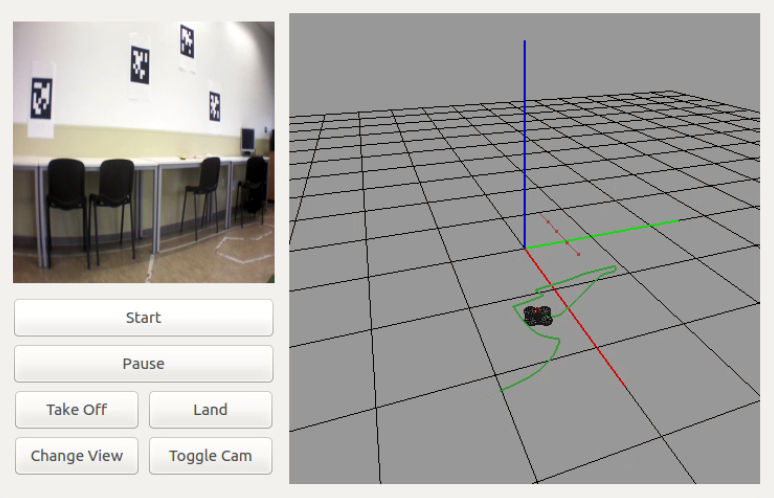
\includegraphics[width=8cm]{img/fullreal1}
	\end{figure}
\end{center}

\end{hslide}


\begin{hslide}
\slsect{Experimentos (II)}
\slsubsect{Sistema completo en entorno real}

\begin{center}
	\begin{figure}
		\centering
		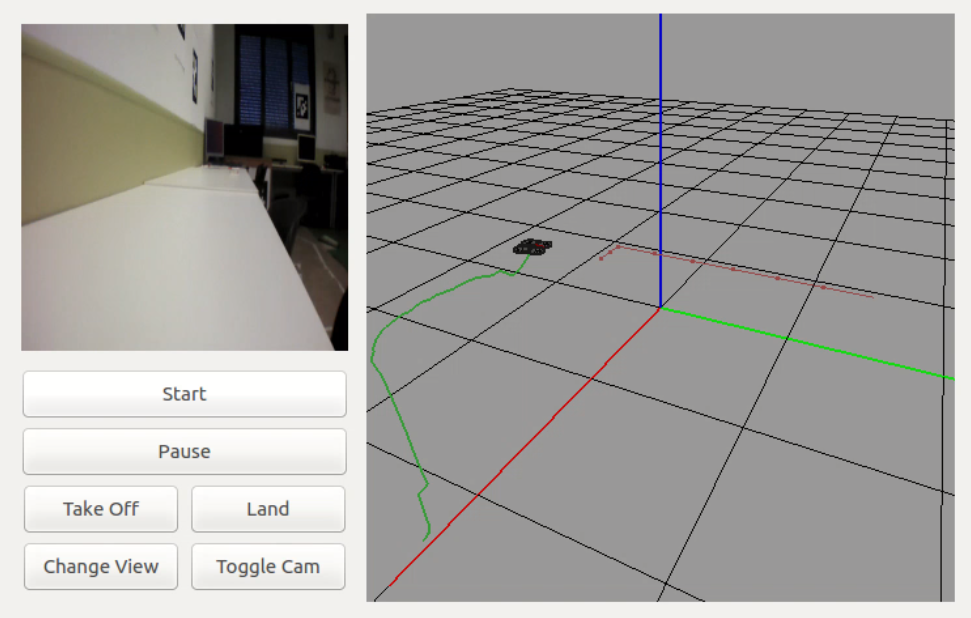
\includegraphics[width=8cm]{img/realderiva}
	\end{figure}
\end{center}

\end{hslide}

\begin{hslide}
\slsect{Experimentos (II)}
\slsubsect{Sistema completo en entorno real}

\begin{center}
	\begin{figure}
		\centering
		\begin{subfigure}
			\centering
			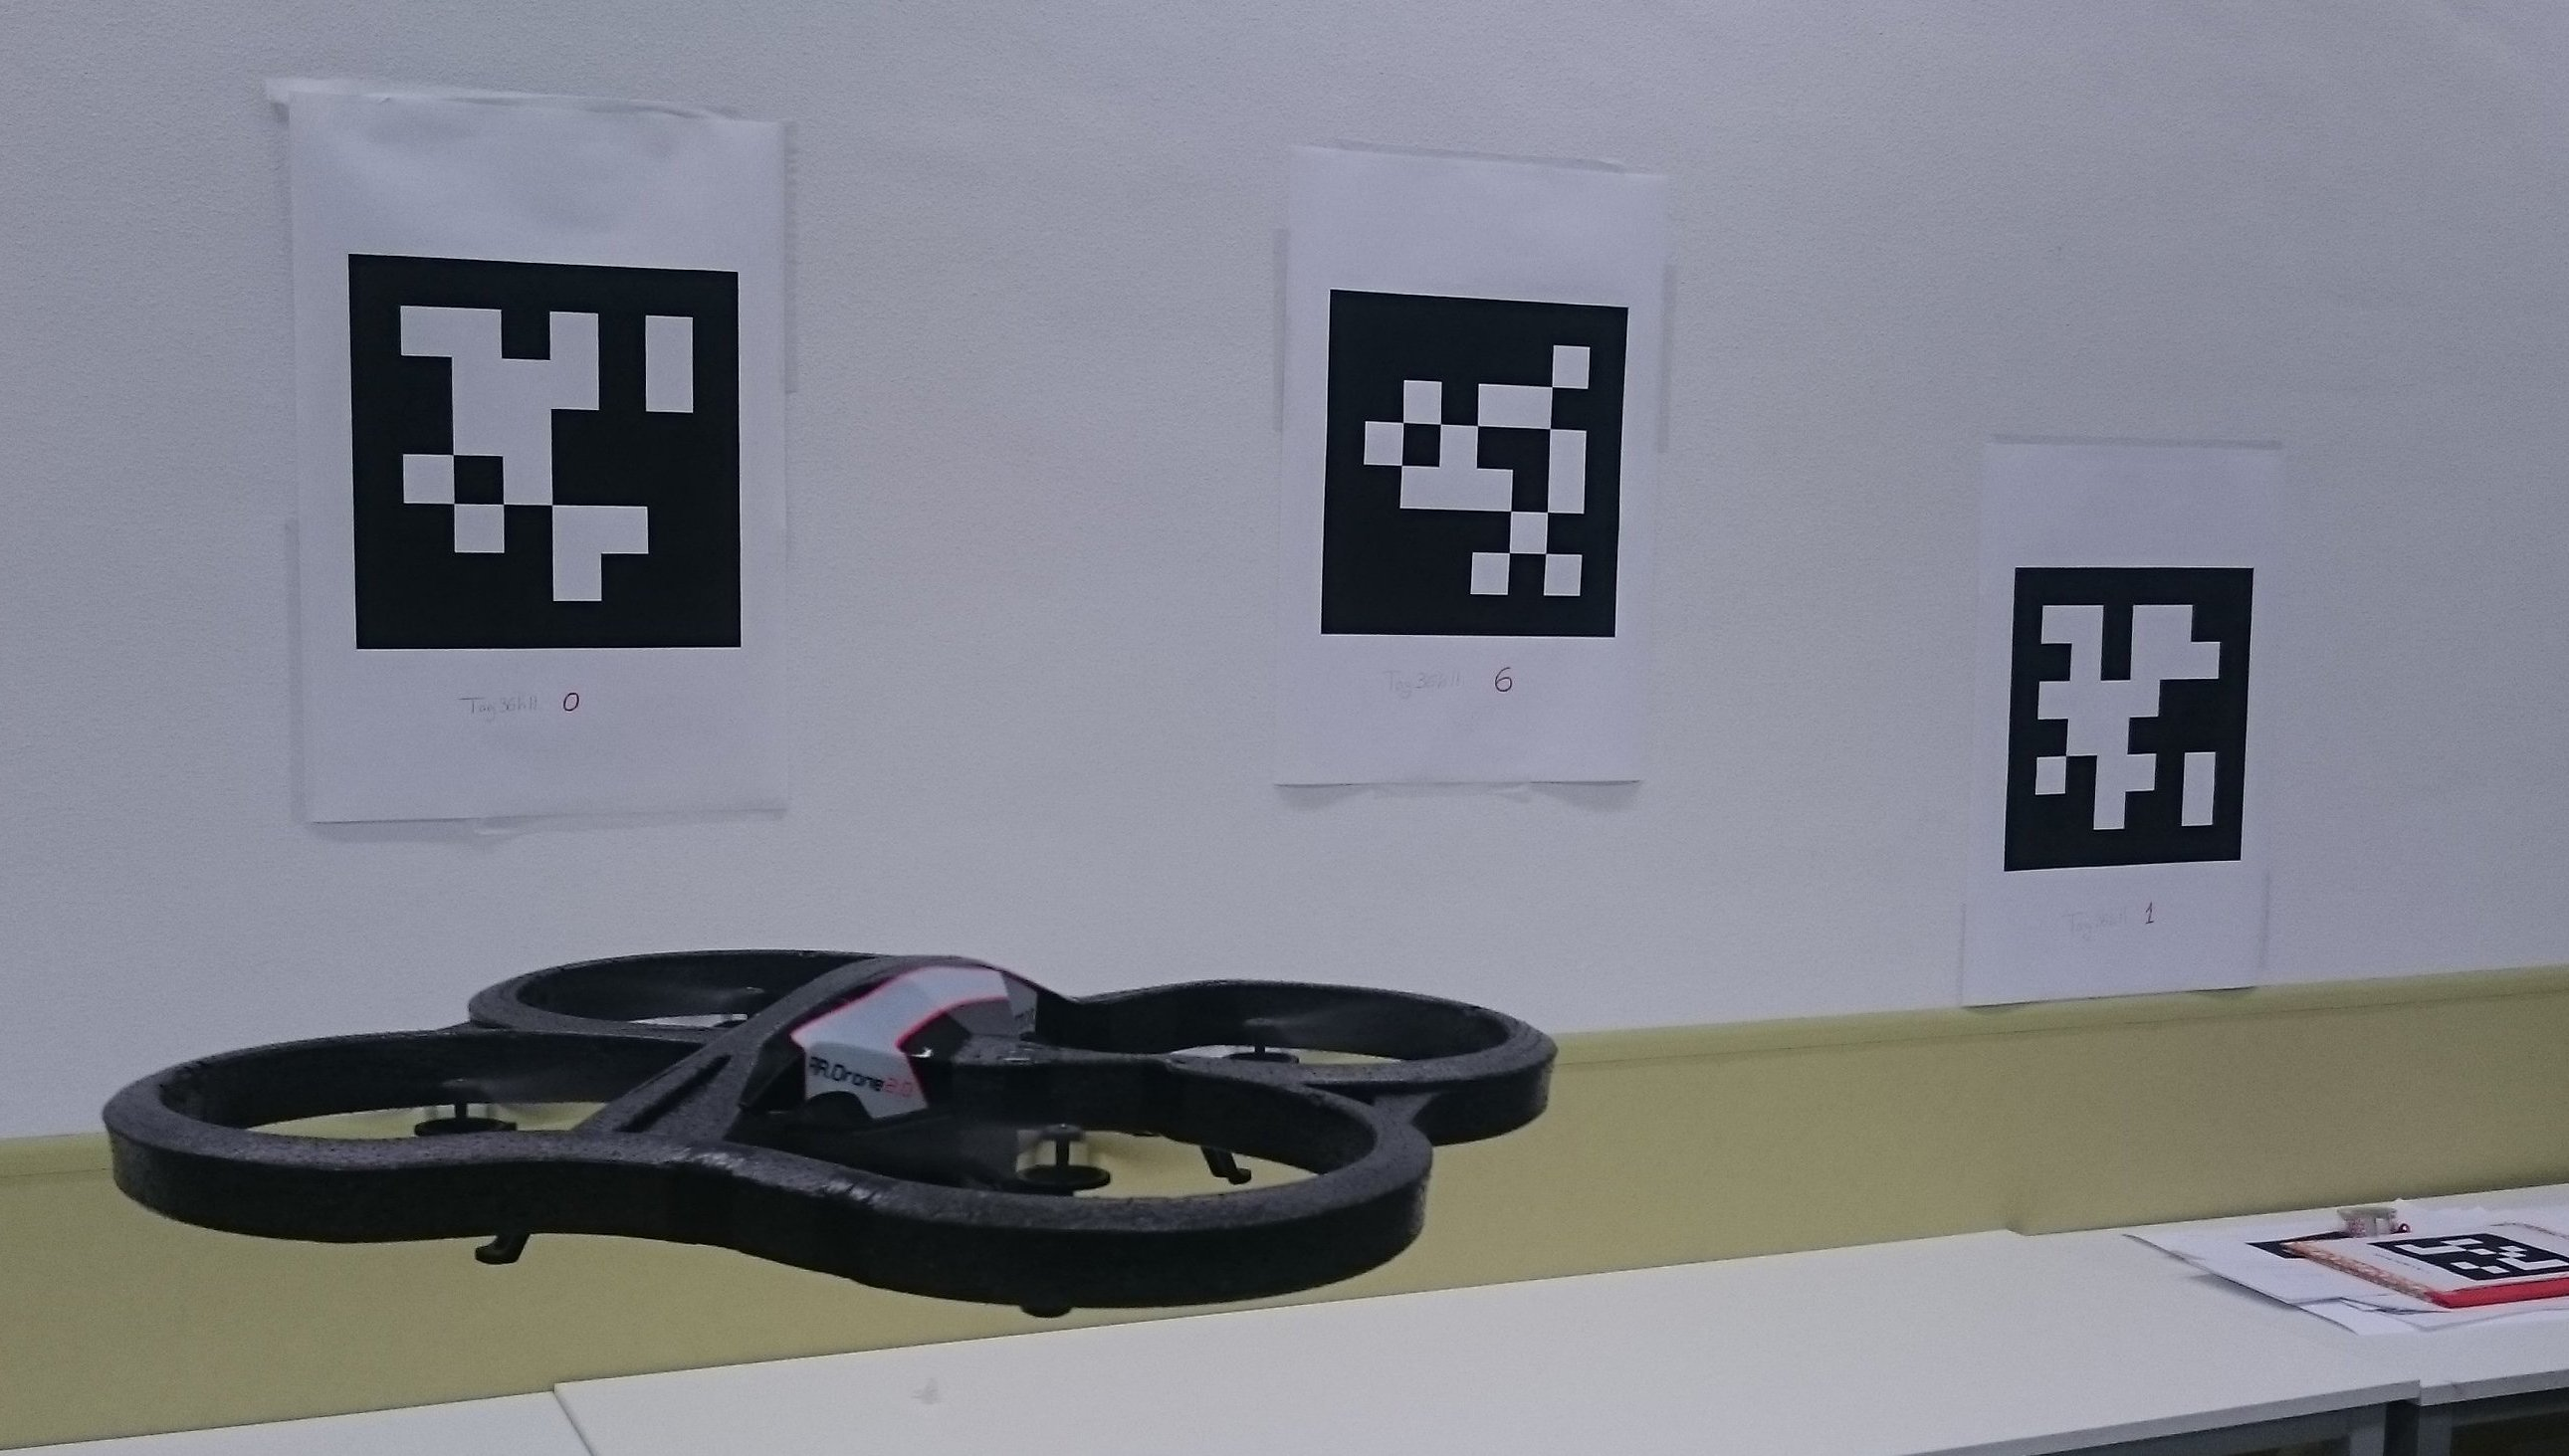
\includegraphics[width=5.5cm]{img/dronevueloreal}
		\end{subfigure}%
		\begin{subfigure}
			\centering
			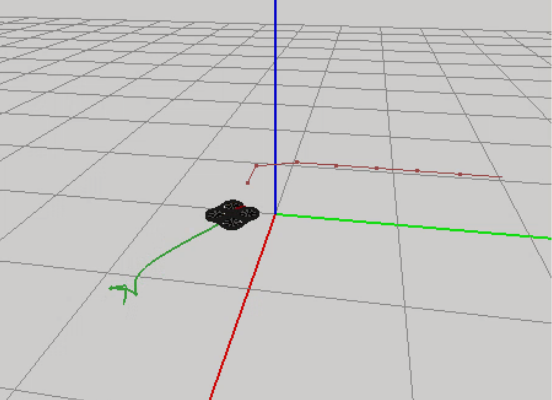
\includegraphics[width=5cm]{img/appcapture}
		\end{subfigure}
	\end{figure}
\end{center}

\end{hslide}



\begin{hslide}
\slsect{Conclusiones (II)}

\begin{itemize}
\item Desarrollo de componente de navegación
\item Refactorización e integración de componente de autolocalización
\item Validación esperimental en simulación
\item \textit{Extra}: Experimentos en entorno real
\end{itemize}

\end{hslide}


\begin{hslide}
\slsect{Conclusiones (II)}
\slsubsect{Trabajos Futuros}

\begin{itemize}
\item Nuevos tipos de movimiento
\item Funcionalidades adicionales
\item Sistema propio de estabilización
\item Técnicas complementarias de visión artificial
\end{itemize}

\end{hslide}

\end{document}